\chapter[变化有了形状：版本与变化本体]{变化有了形状：\\版本与变化本体}

\begin{noteblock}
Semantica 绑定： 本章保存配置、变化、证据保质期与逐项裁决方法；唯一机器语义是
\nolinkurl{semantica.chapter_packages.vol2.ch17}，主场景为
\nolinkurl{semantica.vol2.ch17.scenario.primary}。本体、CQ、查询、Shape、变化/裁决正反案例、
规则、oracle、snapshot/diff、PROV 与 receipt 全部在 Semantica。当前为
\nolinkurl{partial}、release \nolinkurl{blocked}；未登记变化不得被系统静默解释为“无影响”。
\end{noteblock}

\begin{center}
\vspace{0.2em}
\chapterartfade{%
\adjustbox{max size={0.88\linewidth}{0.27\textheight}}{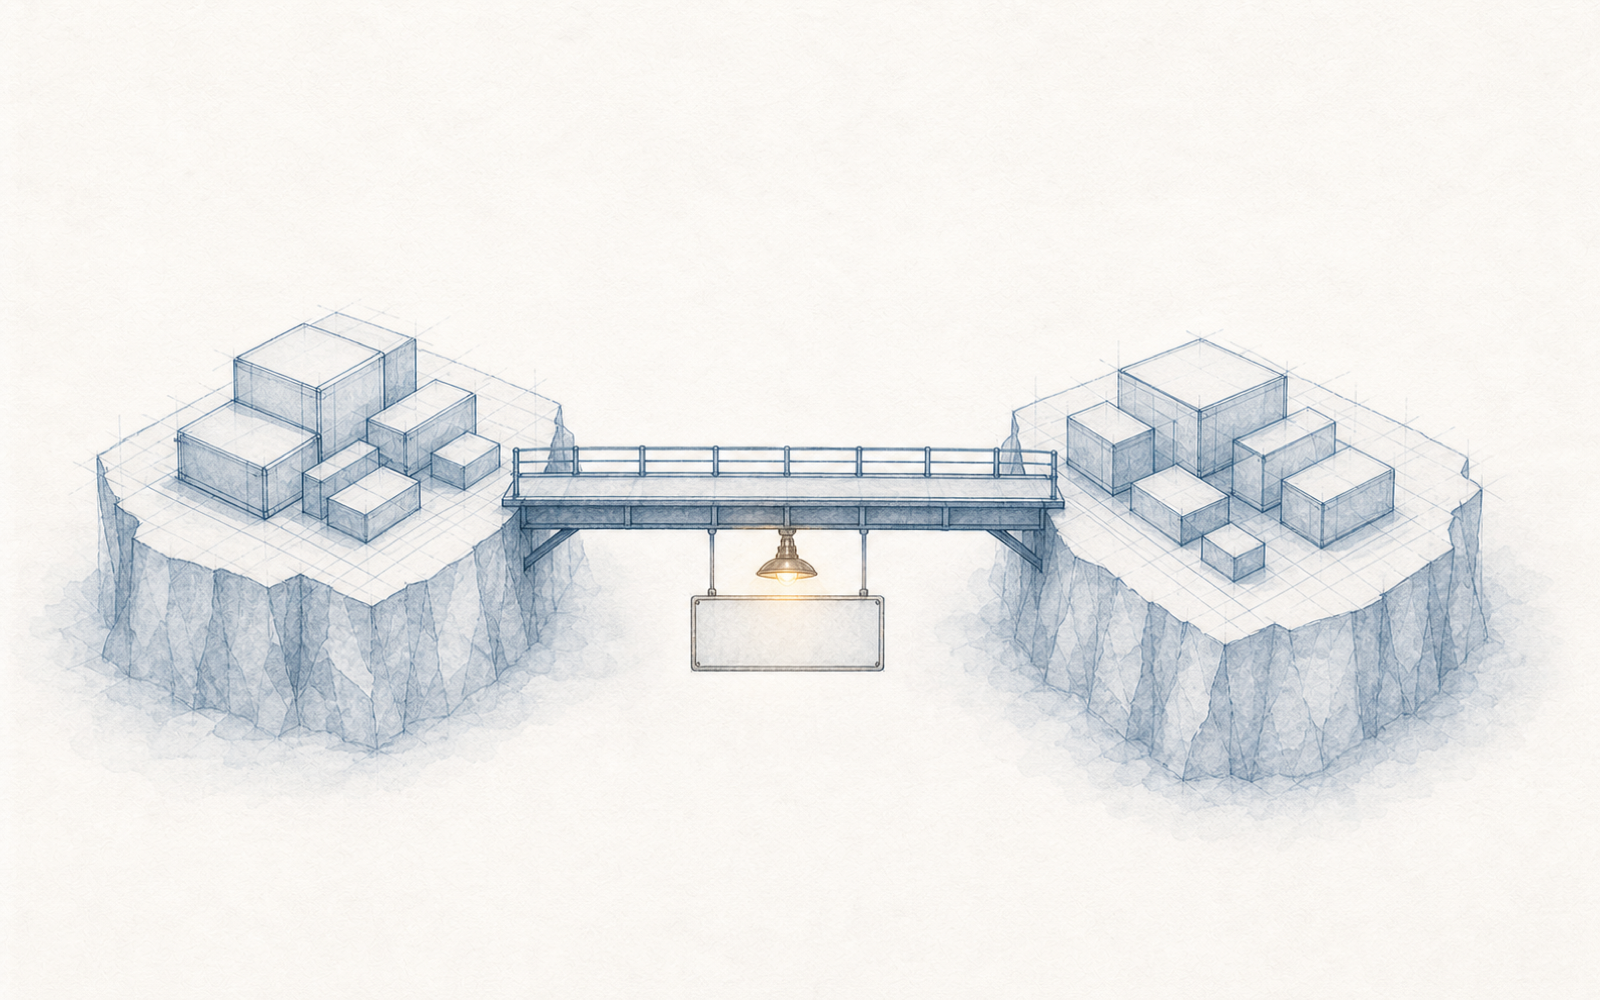
\includegraphics{figures-imagegen/art-ch17-v01.png}}%
}
\vspace{0.35em}
\end{center}

\begin{noteblock}
\textbf{【导读】}
上一章结束时，数字终于都带上了出处：每个值背后站着对象、方法与来源，
证据从来没有这么新鲜过。可散会前小林只补了一句话，就让这份新鲜显得脆弱——
“产品在变。下个月，这些证据还新鲜吗？”第 7 章章末冻结的三个问题由此回到
桌上：怎样让每张“通过”可查地绑定自己的构建、环境与判据，而不是靠人回忆；
一次变更之后，怎样自动列出哪些结论过期、哪些仍在保质期、理由是什么；
时间流逝时，怎样发现悄悄的漂移。本章跟着小蔡给“变化”建一个最小的形状——
快照、维度、事件、差异分析——然后把当年的两场事故在新载体上重演一遍。
读完本章，你应当能把一次变更交给一条查询，让机器回答：哪些“通过”因此
过期、哪些仍在期内——以及更重要的——每一个答案凭什么。
\end{noteblock}

\Needspace{6\baselineskip}
\section{三个问题，等一个形状}

测量那一摊收尾的时候，试点的士气正高：数字进账要带出处的规矩立住了，
吴工那边连最不服气的人都承认，“来历不明的数字进不了账”这道门挡下的
麻烦比它添的麻烦多。可庆功的话音没落，小林就把下一块石头放在了桌上——
证据是新鲜的，产品却在动。变更单在途，工具链在换代，台架在维护升级；
一份今天带足出处的证据，下个月支持的还是不是今天这句话？

试点推进到软件域那天，小林抱来一只文件盒，最上面是那张著名的手工差异分析
表：每行一件回归资产，列上写着它绑定的构建、环境、夹具版本、结论和失效
条件。这张表在评审会上被接受过，今天也仍然是对的——靠他的记忆、他付过的
学费和他的认真。小蔡看完只问了一句：“您休假那两周呢？”小林想了想，给了
一个诚实的回答：“那两周，大家尽量不升版。”没有人笑。一套靠某个人在场才
成立的做法，再对也只是这个人的做法。

小蔡把第 7 章冻结的三个问题翻译成三句机器要接的话，写在白板上：给一张
“通过”，你能回答它绑定的构建、环境与判据吗；给一次变更，你能列出重开
集合并逐项给出理由吗；给一段时间，你能指出哪些绑定物已经悄悄不在了吗。
按团队已经用惯的规矩，这三句话就是本章这个本体的验收边界：它承诺回答
这三问，也只回答这三问——变更该不该批、重测值不值得，都不在它的射程里。

三句话共享同一个前提：机器得先看得见“变了什么”。而此刻“变”在团队手里
只有两种存在方式。一种是代码仓库的逐行差异——太细了，机器看得见每一行，
却不知道哪些行属于软件、哪些牵动标定的解释，更糟的是它根本照不到编译器；
当年那十一天，逐行差异是零，事故照样发生。另一种是变更单——一份写给人
读的文档，“其余声明不变”落在纸上就到了头，第 7 章已经算过这笔账：声明
不变是变更单的义务，验证不变是另一回事，纸面上这两件事之间没有桥。

两条路缺的是同一样东西：变化本身还没有形状。变化，应该长什么样？

\Needspace{6\baselineskip}
\section{变化的形状：快照与事件}

先立快照。第 1 章那张配置清单——硬件、软件、标定、驱动、基线——已经是
快照的雏形，但在纸面上它只是主张里的一个从句，谁引用谁抄写，抄错了没有
任何东西会响。也别指望发布包目录能顶替它：文件夹装得下软件和标定，装不下
“当时用哪套工具链把它们变成机器行为”。现在把清单立成对象：一个配置快照
是一个东西，它有维度，每个维度有值，它可以被引用、被比对、被绑定。小蔡
抄完五行，小林伸手添了第六行：环境。“清单上从来没有它。我为它付过十一天。”

下面这段记法在说什么：把候选 RC17 写成一个六维的快照对象，逐维给值——
\Needspace{8\baselineskip}
注意第六维和前五维平起平坐。

\nopagebreak[4]
\begin{codebox}
\begin{Verbatim}[fontsize=\small,breaklines=true,breakanywhere=true,breaksymbolleft={},breaksymbolright={}]
# 候选 RC17 的配置快照（示意记法）
chg:Snapshot_RC17 a chg:ConfigSnapshot ;
    chg:hardware    chg:HW_H32 ;    # 硬件维：H3.2 控制器
    chg:software    chg:SW_183 ;    # 软件维：SW1.8.3
    chg:calibration chg:Cal_C41 ;   # 标定维：C41
    chg:driverPack  chg:Drv_D7 ;    # 驱动维：D7
    chg:baseline    chg:Base_V12 ;  # 基线维：V12 集成基线
    chg:buildEnv    chg:Env_E7 .    # 环境维：编译器、选项、库、夹具的组合
\end{Verbatim}
\end{codebox}

环境第一次成了配置的正式一维，而不是散落在某人记忆里的背景。快照立成
对象之后，“两个快照相不相同”从眼力活变成了逐维比对——这件小事后面要
派大用场。

再立事件。变化不是“新清单换掉旧清单”的模糊一瞬，而是两个快照之间的
一条边。下面这段记法在说什么：把在途的那次软件升版写成一个变更事件，
\Needspace{8\baselineskip}
边上写明改了哪一维、从什么值到什么值、声明哪些维不动。

\nopagebreak[4]
\begin{codebox}
\begin{Verbatim}[fontsize=\small,breaklines=true,breakanywhere=true,breaksymbolleft={},breaksymbolright={}]
# 一次变更事件：软件维从 1.8.3 升到 1.8.4（示意记法）
chg:Change_0091 a chg:ChangeEvent ;
    chg:fromSnapshot     chg:Snapshot_RC17 ;
    chg:toSnapshot       chg:Snapshot_RC17a ;
    chg:changedDimension chg:software ;   # 改了哪一维
    chg:changedFrom      chg:SW_183 ;
    chg:changedTo        chg:SW_184 ;
    chg:declaresUnchanged chg:hardware , chg:calibration ,
                          chg:driverPack , chg:baseline , chg:buildEnv .
\end{Verbatim}
\end{codebox}

最后那五条“声明不变”不是客套。机器会拿它们与两端快照逐维对表：声明
标定不变、而新快照的标定维实际换了值的事件，登记不进去。变更单上“其余
不变”四个字，第一次从礼貌变成了可核对的承诺。还有一个细节值得指认：
两端快照有五个维度取值相同、只有软件维不同——第 1 章说的“单因变式”，
在这里不再是一句描述，而是两个对象之间可以逐维数出来的事实。

\textbf{变化有了形状：不是两团配置之间的模糊差异，而是两个快照之间一条带名字的边——改了哪一维、声明哪些没动，都写在边上，都可以被对表。}

快照与事件立起来了。可屋里最多的东西既不是快照也不是事件，是历年攒下的
那一摞“通过”。它们站在哪里？

\Needspace{6\baselineskip}
\section{每张“通过”，交代自己的世界}

最省事的办法是给报告模板加三栏：构建、环境、判据。但加栏靠人填，漏填的
报告照样归档，三年后没人分得清空栏意味着“没有”还是“没写”。再省事一点
是靠命名规范和目录结构——文件名装不下六个维度，而且改名无声。两条路都
把“绑定”寄存在自觉上，而本章要防的恰恰是自觉的假期。

新载体的做法只有一条：把每张“通过”登记为对象，绑定即部件，缺件即拒——
第 11 章立下的那条“机器的拒绝比机器的生成值钱”，在这里长出本章的版本。
下面这段记法在说什么：两张“通过”各自写下自己生效的世界——一张是软件
\Needspace{8\baselineskip}
回归，一张是生产写入。

\nopagebreak[4]
\begin{codebox}
\begin{Verbatim}[fontsize=\small,breaklines=true,breakanywhere=true,breaksymbolleft={},breaksymbolright={}]
# 两张“通过”各自绑定的世界（示意记法）
chg:Pass_SwRegression a chg:PassRecord ;
    chg:onSoftware    chg:SW_183 ;   # 生效构建
    chg:onCalibration chg:Cal_C41 ;  # 生效标定
    chg:inEnv         chg:Env_E7 ;   # 生效环境
    chg:byCriterion   chg:Crit_Regression .   # 按什么判据

chg:Pass_MfgWrite a chg:PassRecord ;
    chg:onSoftware    chg:SW_183 ;   # 镜像源于构建——所以老实登记
    chg:inEnv         chg:Env_Line2 ;
    chg:byCriterion   chg:Crit_ImageVerify .
\end{Verbatim}
\end{codebox}

先说这些值从哪里来。登记是一次受控活动：生效构建从流水线的构建记录里
抄，生效环境从工具链清单里抄，谁登记、何时登记都留痕——不允许凭记忆
填写。本体规定“必须有这些部件”，部件的值却必须来自事实的载体；这个
分工本章后面还会回来。

再留意生产写入那一条：它老老实实写下了自己绑定软件维，因为镜像源于构建。
当年的会议室里，它是“最容易被忘掉的重开”；此刻它只是登记表上普通的一行。
这行登记，就是后面一切“不会忘”的全部秘密——先按下不表。判据那一格也
不是摆设：判据本身是对象，它也会改版——判据收紧了一档，旧“通过”
按的还是旧尺子。把判据绑进来，这种更安静的变化才有被问到的一天。

登记到台架那张卡时，屏幕把当年会议室的发现变成了一个可查询的事实：它绑定
的样机、构建、标定三个值，没有一个与目标快照相同。没有人指责这张卡——
它只是永远站在自己的世界里，支持着另一句不在今天桌上的主张。

登记旧档案时也遇到了登记不进去的。团队想起那台 ENV-01：三年前的固件
“通过”还在档案柜里，可构建它的笔记本早已报废，环境维补不出来。缺件即拒
在这里显出它的诚实——补不齐世界的“通过”，不再冒充证据，降级为历史记录。

\textbf{一张“通过”在这个本体里的登记费，是交代自己的全部世界：构建、环境、判据，缺一即拒；交不出世界的“通过”，连过期的资格都没有。}

绑定齐了。走廊尽头的邮件恰好在这时到达——还是那张单子：软件从 1.8.3 升
1.8.4，只改一件事。这一次，重开集合谁来圈？


\begin{noteblock}
\textbf{读图任务}：先找到两组快照蜂窝中的配置差异，再沿下方三张 PASS 卡的锚线回到它们各自属于的快照，最后看哪条锚线已断开。
\end{noteblock}

\begin{center}
\begin{minipage}{\linewidth}
\centering
\adjustbox{max size={\linewidth}{0.78\textheight}}{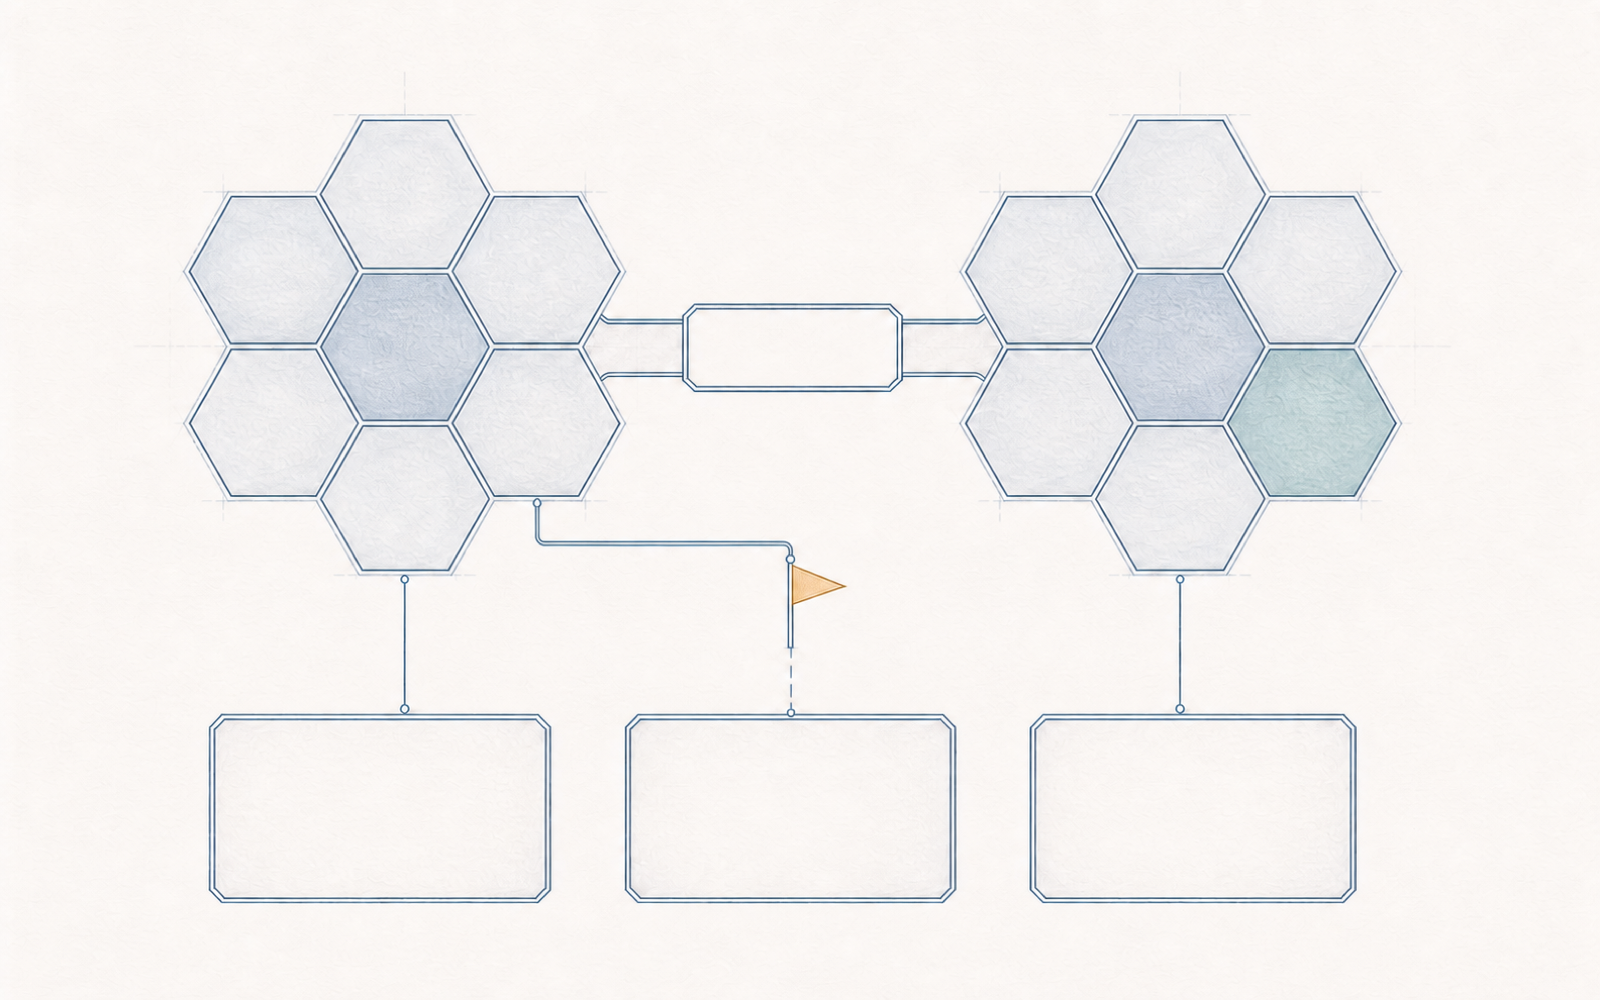
\includegraphics{figures-imagegen/ch17-fig01-snapshot-scoped-pass-v01.png}}
\captionof{figure}{PASS 是带对象、配置、条件和时间的快照结论。快照改变后，旧卡片不必立即变假，但它与当前世界的支持关系必须重新判定。}
\end{minipage}
\end{center}


\begin{noteblock}
\textbf{图后判断}：过期旗只表示需要重开评价，不自动否定原证据，也不表示变更一定导致安全问题。重新通过仍需人员依据差异和影响做决定。
\end{noteblock}

\Needspace{6\baselineskip}
\section{重开集合，由一条查询返回}

这件事团队其实做过两遍。第 1 章的会议室里逐卡辩论了一个下午，得出五张卡
的逐项判决；第 7 章小林的六层清单做得更细，代价是他的记忆和学费。两版
手工清单都对，也都不可复制——换个人、换个星期，就不保证还有这张清单。
至于第三条路，照改动模块机械地圈，它的盲区正是那十一天的出处，早已出局。

\Needspace{8\baselineskip}
现在轮到第四条路。问题：软件维的旧值被换掉之后，哪些“通过”绑定着它？

\nopagebreak[4]
\begin{codebox}
\begin{Verbatim}[fontsize=\small,breaklines=true,breakanywhere=true,breaksymbolleft={},breaksymbolright={}]
SELECT ?pass WHERE {
  chg:Change_0091 chg:changedDimension ?dim ;
                  chg:changedFrom      ?oldValue .
  ?pass a chg:PassRecord ;
        ?binding ?oldValue .           # 这张“通过”绑定了被换掉的旧值
  ?binding chg:bindsDimension ?dim .
}
\end{Verbatim}
\end{codebox}

答案表在一分钟内回来：

\begin{center}
\begingroup\small
\setlength{\tabcolsep}{4pt}
\begin{tabularx}{\linewidth}{@{}XX@{}}
\toprule
查询返回 & 当年的手工对应 \\
\midrule
软件回归卡 & 第 1 章判词：“直接受击” \\
集成冒烟卡 & 第 7 章判词：“新构建整体重做” \\
生产写入卡 & 第 1 章判词：“最容易被忘掉的重开” \\
\bottomrule
\end{tabularx}
\endgroup
\end{center}

生产写入卡回来了，而且没有惊动任何人的记性。机器并不知道镜像是什么、
不知道产线在哪——它只是把登记那天写下的那条绑定原样收了回来。机器不会
忘，不是因为它聪明，是因为它从来不需要记。答案表的第二列同样要紧：
每一行都自带理由——“因为你绑定了被换掉的那个值”。当年两版手工清单给
过同样的判词，但判词长在小林的脑子里；现在它长在返回结果上，谁来问，
答案都一样。

小蔡把返回结果与两版手工清单并排贴在白板上对了一遍账：第 1 章那个下午
辩出来的逐卡判决，第 7 章那张六层表格，凡是冲着绑定去的行，机器全数
命中，一张不多、一张不少——用时一分钟，而那个下午开了三个小时。

台架卡不在返回里，这同样值得看一眼：它绑定的从来不是目标快照的任何旧值，
在新载体里它对新主张本来就没有取得过支持关系——“顺手收编”这一回连门
都找不到。第 1 章它一连教过两课——“对不上表要说明”“接近了也要说明”，
第 7 章升版在即时它把第二课重讲了一遍，这一章它上完了最后一课：
说明不再靠人守着，错位本身就写在绑定里。
而集合之外的概念卡与冲振卡，此刻的身份是“保留候选”，不是“自动保留”
——这个区别马上就要紧起来。

还有一笔账要如实记下：当年会议室圈过硬件卡——它的绿建立在诊断假设上，
软件差异若触及诊断路径，假设就要重新确认。这条查询没有返回它。先把这笔
账记在白板角上，本章结尾要用。

\textbf{重开集合不是谁的记性好，而是绑定关系的必然推论：查询只是把登记那天写下的承诺，原样收回来。}

集合摆上桌，处理它的两种最痛快的办法，立刻有人说出口。

\Needspace{6\baselineskip}
\section{两种痛快，被同一道门拦住}

郑工先开口：“既然机器一分钟就能圈出来，那就干脆点——集合内外一起，全部
作废、全部重测，机器排期，一次洗干净。”这话一点不外行。这是被那年冬天
教育过的人的本能：宁可多测，不可漏测，很多行业的血就是这样止住的；而且
它这回还多了一层底气——重测的账单可以让机器去排，勤奋第一次显得不贵。
对面的痛快也有人记得——“软件而已，旧证据接着用”，那句话的上一个版本
追回过十几辆样车；这回它换了件衣服，在会议室里飘了一句：“查询没圈到的，
照单全收就行了吧。”两句话在第 1 章的会议室里交过一次手，靠的是人的辩论；
这一次，它们要过的是一道结构的门。

新载体给这两种痛快准备的不是反驳，是一个对象。每一份差异分析是一个东西：
一端连着旧证据——那摞“通过”，一端连着关于新快照的新主张，中间是逐项
判决。判决只有两种写法，各带一个必填件：保留，须带理由；作废，须带
波及面——这次作废剥夺了哪些结论的支持，一项项点名。判决写完，差异分析
对象本身也进档案：它不是会议纪要的附件，而是下一次变更的输入——三个月
后再升一版，今天的每条保留理由都会被重新问一遍还成不成立。

先试郑工的“全部作废”。助手照吩咐批量生成判决，跑到冲振卡那行卡住了：
作废判决的波及面是空的——冲振卡绑定的世界没有一维被这次变更触碰，它的
作废剥夺不了任何在场结论的支持。宣布一张卡作废，却说不出作废了谁，这不是
判断，是挥手——门禁拒收。再试“照单全收”：概念卡那行的保留判决缺理由，
同一道门，同样拒收。下面这段记法在说什么：机器怎样拒绝一条没有理由的
\Needspace{8\baselineskip}
“保留”。

\nopagebreak[4]
\begin{codebox}
\begin{Verbatim}[fontsize=\small,breaklines=true,breakanywhere=true,breaksymbolleft={},breaksymbolright={}]
# 门禁：没有理由的“保留”被拒绝（示意记法）
[ a chg:GateReport ;
  chg:violates chg:RetainNeedsReason ;   # 保留须带理由
  chg:focus    chg:Verdict_ConceptCard ; # 概念卡的保留判决
  chg:missing  chg:retainReason ;        # 缺的部件
  chg:message  "保留是判断，不是默认：请写明该卡为何不受本次变更波及" ] .
\end{Verbatim}
\end{codebox}

那行提示语值得慢读：保留是判断，不是默认。概念卡最终当然保留了——理由
是“软件版本不改变相关项边界，安全场景选定经复核未涉软件行为”，这句话
写进判决，成为下次变更时可以被复查、也可以被推翻的东西。逐项判完，
最终的差异分析长这样：查询返回的三张，判重开，各自附着要重跑的范围；
概念卡与冲振卡，判保留，各带一条写下来的理由；台架卡维持原状——它本来
就不曾支持这句主张，无所谓保留或作废。既没有一张卡被顺手处理，也没有
一张卡被勤奋错杀。

\textbf{本体拒绝的不是哪个答案，而是“不逐项”这件事本身：保留是判断，须带理由；作废是判断，须带波及面——两种痛快在这道门前，一样过不去。}

郑工盯着那行拒绝理由看了一会儿，说了三个字：“比我狠。”

“狠”字落在哪儿，值得多想一步。整体判决的诱惑，从来不在省下的工时，
在省下的署名。“全部作废”把判断换成预算——预算是公家的，错杀一张
真证据，不记在任何人名下；“照单全收”把判断换成默认——默认出了事，
账摊在“当时没人反对”上，薄得无人可问。逐项判决贵，贵在每一行后面
都得站一个写理由的人：理由进档案，下次变更还要被重新问一遍成不成立。
两种痛快省掉的是同一样东西——把名字签在具体判断上的成本；这道门
收回来的，也正是这笔账。

这一轮变更被接住了——因为它有变更单。可要是没人递单子呢？

\Needspace{6\baselineskip}
\section{会自己动的那一维}

试点第七周，构建服务器发来例行通知：工具链将于周末升级。当年，这样一封
邮件不会惊动任何人——代码一行没改，编译器又不是产品。小林那十一天的
排查里，所有人都在翻改过的代码，答案却在没人怀疑的地方。纸面世界之所以
查不到，有两层原因：其一，在纸面的变更管理里，编译器升级不算“变更”——
变更单管产品定义，工具链在所有清单之外，没有一张单据为它而设；其二，
旧报告不带环境，“哪些通过依赖旧编译器”这个问题连落笔的地方都没有。

补救的直觉有两个。给作业指导书加一条“工具链升级须评审”？制度靠人记得
触发，而这类升级常由维护脚本在深夜完成。那就冻结工具链、永不升级？
“冻结全世界”的方案第 1 章已经出局过一次，编译器也不例外——安全补丁和
停服日期，不跟项目排期商量。

新载体的回答已经在快照里放好了：环境是第六维，升级就是一次变更事件。
\Needspace{8\baselineskip}
下面这段记法在说什么：把工具链升级登记成一次环境维的变更。

\nopagebreak[4]
\begin{codebox}
\begin{Verbatim}[fontsize=\small,breaklines=true,breakanywhere=true,breaksymbolleft={},breaksymbolright={}]
# 环境也是一维：工具链升级作为变更事件（示意记法）
chg:Env_E8 a chg:BuildEnv ;
    chg:supersedes chg:Env_E7 .        # 升级后的工具链组合
chg:Change_0104 a chg:ChangeEvent ;
    chg:changedDimension chg:buildEnv ; # 改的是环境维
    chg:changedFrom      chg:Env_E7 ;
    chg:changedTo        chg:Env_E8 .
\end{Verbatim}
\end{codebox}

事件登记的那一刻，17.4 那条重开查询换个维度参数照跑，返回绑定旧环境的
每一张“通过”——四百多项用例的软件回归卡赫然在列，虽然代码一行没改。
小林看着名单沉默了几秒：“当年我要这张名单，用了十一天。”注意状态的
措辞：不是“作废”，是“待重判”。标疑是查询的义务，判决仍是差异分析的
义务——逐项纪律原样适用。时序敏感的用例大概率要重跑：新工具把同一份
源码翻成另一副机器码，优化的手法变了，指令的快慢、代码在内存里的位置、
任务之间的相对节拍都可能跟着挪——当年那个“迟到几拍”，走的就是这条路；
纯逻辑比对的用例也许凭理由保留：它们判的是输入输出，不押节拍。但每一行
都得有人写下判词。机器给的从来不是结论，是一份不会漏名字的点名册。

漂移也是同一件事的慢版本，这正是白板上第三句能力问题的着落。夹具改版、
台架软件更新，从不发通知——但它们在环境对象里都有名字，任何一个换代
登记进来，绑定旧值的“通过”就会在下一次例行核对里自己浮出水面；反过来，
一张“通过”绑定的环境如果已经不是现行世界里的任何一个成员，它就站在一个
不复存在的世界上，核对会把它标出来——这正是当年 ENV-01 档案柜里那份
报告的处境，只是这一次不用等到出事才发现。发现漂移不再靠小林休假归来的
不安，而是把“现行世界”与“各张通过绑定的世界”定期对表。十一天与
一分钟之间，隔着的不是算力，是一条登记纪律。

\textbf{在纸面世界，环境升级不算变更，因为没有一张单据为它而设；在这个本体里，环境是快照的一维——它一动，绑定它的每一张“通过”当场知道。}

登记、查询、起草判决，这些活助手都干得又快又好。那么人还剩下什么？

\Needspace{6\baselineskip}
\section{助手圈得出集合，签不了字}

差异分析定稿那天，值得把完整的一圈记下来。提议：助手依查询结果起草逐项
判决，把每张卡的绑定、被触碰的维度、建议判决和理由草稿排成一列，末尾
还附了一条自作聪明的建议——台架卡如今装着 1.8.4 的前身，“与新快照高度
接近，建议收编为支持证据”。校验：门禁拒绝，“接近”不是任何一个绑定
谓词，台架卡的三个维度值与新快照逐维对表，零匹配；理由写得再流畅，也
改不动对表的结果——当年要靠小林的判词才能挡住的诱惑，如今在结构上就
进不了门。小唐在旁边看得心痒：“草稿都这么齐了，让它顺手把判决也定了
呗，反正门禁把着关。”小林摇头——门禁把的是“判决不缺件”，从来没把过
“判决是对的”；这两件事之间的距离，恰好是人的位置。执行：被人改定的
判决作为受控活动写入记录，签发人是小林，不是助手。审计：助手的原始提议
连同那次被拒一起留在档案里——下次再有人起“顺手收编”的念头，会先撞见
这条前科。

这一圈里，三种权威各归各位。软件维从什么值变到什么值，是构建系统与变更
记录给出的事实，助手复述它们，不制造它们；什么叫过期、保留缺什么部件，
是本体给出的语义；而“这几张卡本周重测、预算从哪里出、重测前产线暂停
几天”，是小林提、陈工批的决定——门禁报告上，没有留给机器的签名栏。

也要诚实地数一数本体没有做到的事。它不知道 1.8.4 里改了哪两个模块——
那是变更记录的事实；它读不出一条保留理由的好坏——“冲振卡与软件维无涉”
是否成立，靠小林和评审人的工程判断，本体只保证这句话必须存在、必须落在
指定的部件里；它更保证不了登记是全的——它拦得住缺件的登记，拦不住没有
发生的登记。变化的形状让机器接住了两场旧事故，但形状不制造事实，也不
拥有决定。

\Needspace{6\baselineskip}
\section{查得动的绑定，查不动的缝}

散会后，小蔡走回白板，看着角上 17.4 记下的那笔账：这条查询没有返回硬件
卡。当年会议室凭什么圈到它？凭有人知道“硬件分析的绿建立在诊断假设上，
而诊断假设依赖软件的行为”。生产写入卡能被机器找回来，是因为登记那天
写下了“镜像源于软件维”这条绑定；而“假设依赖软件行为”这条边，从来
没有人写下——它不在六个维度里，它是两个专业之间的一条缝。

小林在门口停了停，像是想起了什么：“当年编译器那次，真正出事的也不是
编译器——是两个任务的相对节拍。共享的芯片、共用的电源、同一个时钟，
变化就是顺着这些缝流过去的。你的查询查得动写下来的绑定，查不动没画出来
的缝。”他顿了顿，补了一句当年吴工在门口问过的话的回声：“各自合格，
合在一起就安全吗——现在这个问题轮到机器来接了。”

小蔡在白板角上，把那笔账正式写成了一句话，作为交给下一段路的题目：查询
的射程，止于登记过的绑定。这不是本章的失败——生产写入卡与四百多项用例
证明了登记过的世界有多可靠——而是它诚实的边界：六个维度描述的是一个
配置由什么组成，描述不了各个部分之间怎样互相牵动。

这就是本章交出的账：变化有了形状，重开集合有了查询，两种痛快被挡在了门
外——但变化沿依赖传播，而依赖得先看得见。第 18 章从这里开始：把方框
之间的缝，画成机器能查的边。

导读的承诺现在兑现。合上书之前，做三件事：找一份你手头最近的“通过”
报告，试着为它补出六维快照——补不出来的那几维，就是你的 ENV-01 时刻；
下一次变更单到达时，先别开会，写下“若绑定齐全，查询应返回哪些结论”，
再与会议结果对照，看谁漏了谁；回想你们上一次“全部作废”或“照单全收”，
数一数哪张作废的卡说不出波及面、哪张保留的卡说不出理由——那些说不出的
地方，就是本章那道门要拦的地方。


\begin{noteblock}
\textbf{本章注记}：本章的人物、会议、事故经过与全部产品数字（候选代号、软硬件
版本、标定编号、环境与工具链代号、用例数、排查天数等）均为合成教学材料，
不对应任何真实企业、真实产品或真实个人；文中对变更管理与配置管理做法的
转述为自然语言概括，不构成对任何实际系统的判定或放行结论。各段记法只是
教学投影；唯一可执行版本是 \nolinkurl{semantica.chapter_packages.vol2.ch17}，当前为
\nolinkurl{partial}、release \nolinkurl{blocked}。
\end{noteblock}
